\section{The arithmetic graph and its path grammar}\label{sec:graph}

Throughout, $r_N=(N+1)^2/N=N+2+1/N$ for $N\ge1$. The sequence $r_1=4<r_2=\tfrac92<r_3=\tfrac{16}{3}<\cdots$ is strictly increasing, $r_N>4$ for $N\ge2$, and $r_N$ is in lowest terms ($\gcd(N,(N+1)^2)=1$), so the denominator of $r_N$ is $N$.

\begin{definition}\label{def:G}
$G$ is the graph on $\N$ with edge set $\{\{kN,k(N+1)^2\}:k,N\ge1\}$.
\end{definition}

\begin{lemma}[Edge labels and adjacency test]\label{lem:edges}
(a) Every edge $\{u,v\}$, $u<v$, has a unique representation $u=kN$, $v=k(N+1)^2$; here $k=\gcd(u,v)$ and $N=u/k$.
(b) Integers $u<v$ are adjacent iff $v/g=(u/g+1)^2$ where $g=\gcd(u,v)$.
\end{lemma}
\begin{proof}
If $u=kN$, $v=k(N+1)^2$ then $\gcd(N,(N+1)^2)=1$ gives $\gcd(u,v)=k$, hence $N=u/k$ is determined. This is (a), and it proves ``$\Rightarrow$'' in (b) since $u/g=N$, $v/g=(N+1)^2$. Conversely, if $v/g=(u/g+1)^2$ put $k=g$, $N=u/g$. \qedhere
\end{proof}

\paragraph{Moves.}
For $N\ge1$ and $x\in\N$ define the partial maps $U_N(x)=x\,r_N$ (defined iff $N\mid x$) and $D_N(x)=x/r_N$ (defined iff $(N+1)^2\mid x$). By Lemma~\ref{lem:edges}, $y$ is adjacent to $x$ iff $y=U_N(x)$ or $x=U_N(y)$ for some $N$, and the label $N$ of the edge is unique.

\begin{proposition}[Degree]\label{prop:degree}
$\deg(x)=\tau(x)+\#\{d\ge2:d^2\mid x\}$, where $\tau$ is the number of divisors.
\end{proposition}
\noindent\emph{Source.} The degree formula is established in U2-TI-DYN~\cite{UTI}; the proof below is self-contained.
\begin{proof}
The up-neighbours are $U_N(x)$ for the $\tau(x)$ divisors $N$ of $x$; they are distinct since $N\mapsto r_N$ is injective. The down-neighbours are $D_N(x)$ with $(N+1)^2\mid x$, i.e.\ $d=N+1\ge2$ with $d^2\mid x$; again distinct. Up-neighbours exceed $x$, down-neighbours are smaller, so the two sets are disjoint. \qedhere
\end{proof}

\paragraph{Valuation law.}
For a prime $p$, $v_p(U_N x)=v_p(x)+2v_p(N+1)-v_p(N)$. Put $\tau_N=(2v_p(N+1)-v_p(N))_p\in\Z^{(\mathrm{primes})}$; then $U_N$ adds $\tau_N$ to the valuation vector of $x$ and $D_N$ subtracts it, and $N\mapsto\tau_N$ is injective because $\tau_N$ encodes $r_N$.

\begin{definition}[Path grammar]
The alphabet is $\mathcal A=\{U_N,D_N:N\ge1\}$. A \emph{path} from $x$ is a word $a_1a_2\cdots a_n$ over $\mathcal A$ such that each $a_i$ is defined at $a_{i-1}\cdots a_1(x)$. It is \emph{nonbacktracking} (NB) if no factor $U_ND_N$ or $D_NU_N$ occurs. Paths of $G$ are in bijection with walks in $G$ starting at $x$, and NB paths with NB walks.
\end{definition}

\begin{lemma}[Closure]\label{lem:closure}
If $a_1\cdots a_n$ is a path from $x$ returning to $x$, with $a_i\in\{U_{N_i},D_{N_i}\}$ and signs $\varepsilon_i=\pm1$ ($+$ for $U$), then $\sum_i\varepsilon_i\tau_{N_i}=0$ and $\prod_i r_{N_i}^{\varepsilon_i}=1$. In particular the multiset of labels with sign $+$ and with sign $-$ define equal products of the numbers $r_N$.
\end{lemma}
\begin{proof}
Each move multiplies the current vertex by $r_{N_i}^{\varepsilon_i}$. \qedhere
\end{proof}

\begin{proposition}[Forward paths]\label{prop:forward}
A forward path (only $U$'s) is strictly increasing; its length from $x$ inside any finite subgraph $H\subseteq G$ is at most $|V(H)|-1$. In particular a finite subgraph has no periodic directed forward orbit and the set of forward paths in $H$ has zero entropy.
\end{proposition}
\begin{proof}
$U_N(x)=xr_N\ge 4x>x$. A forward path in $H$ visits distinct vertices, so it has at most $|V(H)|-1$ steps; hence the number of forward paths of length $n$ is $0$ for $n\ge|V(H)|$. \qedhere
\end{proof}

\section{Nonbacktracking histories}\label{sec:nb}

Let $H$ be a graph. A \emph{directed edge} is an ordered pair $(u,v)$ with $\{u,v\}\in E(H)$; write $\vec E(H)$ for the set of directed edges and $\bar e=(v,u)$ for the reverse of $e=(u,v)$. The \emph{edge matrix} (Hashimoto matrix~\cite{Ha,Ba}) $B_H\in\{0,1\}^{\vec E\times\vec E}$ has $B_H(e,e')=1$ iff $e=(u,v)$, $e'=(v,w)$ and $w\ne u$. A \emph{nonbacktracking walk} of length $n$ is a sequence $e_1\cdots e_n$ with $B_H(e_i,e_{i+1})=1$. The set of bi-infinite NB walks is the edge shift $X_{\mathrm{NB}}(H)$ of the $0$--$1$ matrix $B_H$; for finite $H$ its topological entropy is
\[
\hNB(H)=\lim_{n\to\infty}\tfrac1n\log\one^{\!\top}B_H^{\,n-1}\one=\log\rho(B_H)
\]
(Lind--Marcus~\cite{LM}). We use the following elementary facts repeatedly.

\begin{lemma}[Positive eigenvector bounds]\label{lem:CW}
Let $B\ge0$ be a square matrix and $\varphi>0$ a vector. Then $\min_i(B\varphi)_i/\varphi_i\le\rho(B)\le\max_i(B\varphi)_i/\varphi_i$. If $B\varphi=\lambda\varphi$ then $\rho(B)=\lambda$ and, for all $n\ge0$,
\[
\lambda^{n}\,\frac{\one^\top\varphi}{\max_i\varphi_i}\;\le\;\one^\top B^n\one\;\le\;\lambda^n\,\frac{\one^\top\varphi}{\min_i\varphi_i}.
\]
No irreducibility is needed.
\end{lemma}
\begin{proof}
The first statement is the Collatz--Wielandt inequality (Horn--Johnson~\cite{HJ}, Section~8.1). If $B\varphi=\lambda\varphi$ both bounds equal $\lambda$. For the last display, $\one\le\varphi/\min\varphi$ entrywise gives $\one^\top B^n\one\le\one^\top B^n\varphi/\min\varphi=\lambda^n\one^\top\varphi/\min\varphi$, and similarly from $\one\ge\varphi/\max\varphi$. \qedhere
\end{proof}

\begin{lemma}[Monotonicity and degree bound]\label{lem:mono}
If $H'\subseteq H$ then $\hNB(H')\le\hNB(H)$. If $\Delta$ is the maximal degree of a finite graph $H$ then $\hNB(H)\le\log(\Delta-1)$ for $\Delta\ge2$.
\end{lemma}
\begin{proof}
$B_{H'}$ is a principal submatrix of $B_H$, so $\rho(B_{H'})\le\rho(B_H)$. Each NB step has at most $\Delta-1$ continuations, so $\one^\top B^{n-1}\one\le|\vec E|(\Delta-1)^{n-1}$. \qedhere
\end{proof}

\paragraph{Countable graphs.}
For the infinite graph $G$ the NB shift $X_{\mathrm{NB}}(G)\subseteq\vec E(G)^{\Z}$ is a countable-alphabet shift. Following Gurevich~\cite{Gu} (and the convention E2 of~\cite{UENT}) we use the \emph{finite-subsystem capacity}
\[
\Hfin(G)=\sup\{\hNB(F):F\subseteq G\text{ finite subgraph}\}=\sup_{F}\log\rho(B_F).
\]
By Lemma~\ref{lem:mono}, for any exhaustion of $G$ by finite subgraphs $F_1\subseteq F_2\subseteq\cdots$ the limit of $\hNB(F_j)$ is $\Hfin(G)$.

\paragraph{The metric shift $Y_{\mathrm{NB}}$.}
The inherited construction of~\cite{USTAGE,UENT} (the shift $Y_{\mathrm{NB}}$ is defined in~\cite{USTAGE}, where its equivalence with nonbacktracking walks is also recorded) uses vertex sequences $(v_i)$ in a window $H=G[V]$ with consecutive vertices adjacent and pairwise distances $(d(v_i,v_{i+1}),d(v_{i+1},v_{i+2}),d(v_i,v_{i+2}))=(1,1,2)$. If $H$ is triangle-free (true for every induced subgraph of $G$ by Theorem~\ref{thm:cycles}), then $d_H(v_i,v_{i+2})=2$ iff $v_i\ne v_{i+2}$, because $v_i,v_{i+2}$ cannot be adjacent. Hence $Y_{\mathrm{NB}}(H)$ is exactly the set of NB walks of $H$, written as vertex sequences; the vertex and directed-edge descriptions are bijective for simple graphs. In particular $h(Y_{\mathrm{NB}}(H))=\hNB(H)$.

\section{Cycles and periodic symbolic paths}\label{sec:cycles}

\begin{theorem}[Cycle structure of $G$]\label{thm:cycles}
\begin{enumerate}[label=(\roman*),itemsep=1pt]
\item $G$ is triangle-free.
\item $G$ has girth $4$: the vertices $2,8,36,9$ form a $4$-cycle.
\item $G$ has odd girth $5$: $6,24,96,784,27$ form a $5$-cycle.
\item For every $x$ and every divisor $N\ge2$ of $x$, the vertices $x,\;4x,\;4xr_N,\;xr_N$ form a $4$-cycle (a \emph{scaling square}); it corresponds to the relation $r_1r_N=r_Nr_1$.
\item Four-cycles do not all involve $N=1$: the vertices $6,27,144,32$ form a $4$-cycle with labels $N=2,3,2,3$ (the commuting moves $U_2$ and $U_3$, relation $r_2r_3=r_3r_2$).
\end{enumerate}
\end{theorem}
\noindent\emph{Source.} Triangle-freeness (i) and odd girth $5$ (iii) were proved in U3~\cite{UTHREE}. The girth $4$ in (ii) is the correction recorded in U3-COR~\cite{UCOR}; it is not stated in the original U3 release. The proofs below are self-contained.
\begin{proof}
(i) A triangle $u<v<w$ has edge labels $a$ (for $uv$), $b$ ($vw$) and $c$ ($uw$), so $r_ar_b=r_c$, i.e.\ $c(a+1)^2(b+1)^2=ab(c+1)^2$. Multiplying by $c$ gives $\bigl(c(a+1)(b+1)\bigr)^2=abc\,(c+1)^2$, so $abc=h^2$ is a perfect square with $h>0$ an integer and $c(a+1)(b+1)=h(c+1)$. Since $\gcd(c,c+1)=1$, $c\mid h$; write $h=ct$. Then $ab=ct^2$ and $(a+1)(b+1)=t(c+1)$. Expanding, $ct^2+a+b+1=tc+t$, hence
\[
a+b=(t-1)(1-ct)\le0,
\]
because $t\ge1$, $c\ge1$. This contradicts $a,b\ge1$.

(ii) The edges are $\{2,8\}$ ($k=2,N=1$), $\{8,36\}$ ($k=4,N=2$), $\{9,36\}$ ($k=9,N=1$) and $\{2,9\}$ ($k=1,N=2$). With (i), the girth is $4$.

(iii) The edges are $\{6,24\}$ ($k=6,N=1$), $\{24,96\}$ ($k=24,N=1$), $\{96,784\}$ ($k=16,N=6$: $16\cdot6=96$, $16\cdot49=784$), $\{27,784\}$ ($k=1,N=27$) and $\{6,27\}$ ($k=3,N=2$). Together with (i), the shortest odd cycle has length $5$. The cycle encodes $r_1r_1r_6=r_2r_{27}$ (both sides equal $784/6$).

(iv) The four edges are $\{x,4x\}$ ($k=x,N=1$), $\{x,xr_N\}$ ($k=x/N$), $\{4x,4xr_N\}$ ($k=4x/N$), $\{xr_N,4xr_N\}$ ($k=xr_N,N=1$); the four vertices are distinct because $r_N>4$.

(v) The edges are $\{6,27\}$ ($k=3,N=2$), $\{27,144\}$ ($k=9,N=3$), $\{32,144\}$ ($k=16,N=2$) and $\{6,32\}$ ($k=2,N=3$). \qedhere
\end{proof}


\begin{proposition}[Relations and closed walks]\label{prop:relations}
Let $w=a_1\cdots a_n$ be a word over $\mathcal A$, $a_i\in\{U_{N_i},D_{N_i}\}$ with signs $\varepsilon_i$, and let $x\in\N$.
\begin{enumerate}[label=(\alph*),itemsep=1pt]
\item If $w$ is a closed path at $x$, then $\prod_ir_{N_i}^{\varepsilon_i}=1$ (Lemma~\ref{lem:closure}).
\item Conversely, if $w$ is \emph{admissible} at $x$ (each $a_i$ is defined at the vertex reached) and $\prod_ir_{N_i}^{\varepsilon_i}=1$, then $w$ is a closed path at $x$. It is a cycle iff $n\ge3$ and the $n$ vertices $x,a_1(x),\dots,a_{n-1}\cdots a_1(x)$ are distinct.
\item Admissibility is not implied by the relation: the relation $r_1r_N=r_Nr_1$ holds for every $N$, but the word $U_1U_ND_1D_N$ is admissible at $x$ iff $N\mid x$.
\end{enumerate}
\end{proposition}
\begin{proof}
(a) was proved in Lemma~\ref{lem:closure}. (b) The vertex reached is $x\prod_ir_{N_i}^{\varepsilon_i}=x$, and a closed walk is a cycle iff its vertices are distinct and $n\ge3$. (c) The word applied to $x$ gives successively $4x$, $4xr_N$ (needs $N\mid4x$), $xr_N$ (needs $4\mid4xr_N$, i.e.\ $xr_N\in\N$, i.e.\ $N\mid x$ since $\gcd(N,(N+1)^2)=1$), and $x$. If $N\mid x$ all steps are defined; if $N\nmid x$ the third step is undefined (for instance $x=2$, $N=4$: $2\to8\to50\to50/4\notin\N$). \qedhere
\end{proof}

\begin{figure}[t]
\centering
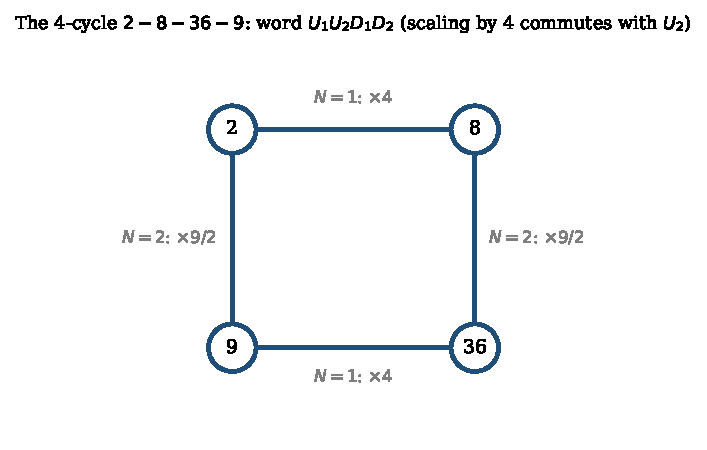
\includegraphics[width=0.62\textwidth]{../figures/fig1_four_cycle.pdf}
\caption{The girth-$4$ cycle $2\!-\!8\!-\!36\!-\!9$, the scaling square of $x=2$, $N=2$. Opposite edges carry equal labels, reflecting the commutation $r_1r_2=r_2r_1$ of the two moves.}\label{fig:four}
\end{figure}

The picture behind Theorem~\ref{thm:cycles}(iv) is that scaling by $4$ ($N=1$) commutes with every up-move $U_N$ for which both orders are defined: every divisor $N\ge2$ of $x$ gives a square on the common edge $\{x,4x\}$. The next section studies the graph obtained by gluing all these squares along that edge.

\section{Exact entropy of theta graphs}\label{sec:theta}

A \emph{theta graph} $\Theta(\ell_1,\dots,\ell_s)$, $s\ge2$, consists of two vertices $u,v$ (the hubs) and $s$ internally disjoint paths of lengths $\ell_1,\dots,\ell_s\ge1$ joining them, at most one of which has length $1$ (so the graph is simple). For $s=2$ it is a cycle.

Directed edges of $\Theta$ are of two kinds: $e_{i,t}$, the $t$-th edge of path $i$ traversed from $u$ towards $v$ ($1\le t\le\ell_i$), and $f_{i,t}$, the $t$-th edge of path $i$ traversed from $v$ towards $u$. The edge matrix is given by $e_{i,t}\to e_{i,t+1}$, $f_{i,t}\to f_{i,t+1}$ ($t<\ell_i$), and, at the hubs,
\[
e_{i,\ell_i}\to f_{j,1}\quad(j\ne i),\qquad f_{i,\ell_i}\to e_{j,1}\quad(j\ne i).
\]

\begin{theorem}[Entropy of theta graphs]\label{thm:theta}
Let $s\ge3$. Then $\rho(B_\Theta)$ is the unique $\lambda>1$ with
\[
\sum_{i=1}^s\frac1{\lambda^{\ell_i}+1}=1,
\]
and the edge matrix has a positive eigenvector for this $\lambda$.
\end{theorem}
\begin{proof}
The function $f(\lambda)=\sum_i(\lambda^{\ell_i}+1)^{-1}$ is strictly decreasing on $[1,\infty)$ with $f(1)=s/2\ge3/2>1$ and $f(\lambda)\to0$, so a unique root $\lambda>1$ exists. Put $c_i=(\lambda^{\ell_i}+1)^{-1}$, so that $\sum_ic_i=1$ by the choice of $\lambda$, and define
\[
\varphi(e_{i,t})=\varphi(f_{i,t})=\lambda^{t-1}c_i>0 .
\]
For $t<\ell_i$: $(B\varphi)(e_{i,t})=\varphi(e_{i,t+1})=\lambda\varphi(e_{i,t})$. For the last edge, $(B\varphi)(e_{i,\ell_i})=\sum_{j\ne i}\varphi(f_{j,1})=\sum_{j\ne i}c_j=1-c_i$ (using $\sum c_j=1$), while $\lambda\varphi(e_{i,\ell_i})=\lambda^{\ell_i}c_i=1-c_i$ because $(\lambda^{\ell_i}+1)c_i=1$. The same holds for $f$. Thus $B\varphi=\lambda\varphi$ with $\varphi>0$, and Lemma~\ref{lem:CW} gives $\rho(B)=\lambda$. \qedhere
\end{proof}

\begin{corollary}[Comparisons]\label{cor:theta}
(a) If all lengths equal $\ell$ ($s\ge3$ paths), $\rho(B_\Theta)=(s-1)^{1/\ell}$.
(b) $\rho(B_\Theta)$ is strictly decreasing in each $\ell_i$.
(c) For $m\ge2$, $\rho(B_{\Theta(3^{m+1})})=m^{1/3}<\lambda_m=\rho(B_{\Theta(1,3^m)})$: shortening one path of a $\Theta(3^{m+1})$ to length $1$ raises the entropy from $\tfrac13\log m$ to $\log\lambda_m$.
\end{corollary}
\begin{proof}
(a) The equation is $s/(\lambda^\ell+1)=1$. (b) $f(\lambda)=\sum_i(\lambda^{\ell_i}+1)^{-1}$ is strictly decreasing in $\lambda>1$ and strictly decreasing in each $\ell_i$ there; increasing $\ell_i$ lowers $f$, so the root $f=1$ moves to the left. (c) Apply (a) with $\ell=3$, $s=m+1$, and (b) to lengths $(3,3^m)\to(1,3^m)$. \qedhere
\end{proof}

\begin{example}[$\Theta(1,3,3)$, the graph $F_2$ in full]\label{ex:F2}
With $m=2$ the equation $\lambda^3-\lambda^2+\lambda=2$ has root $\lambda_2=1.353210\ldots$ The graph has $7$ edges, hence $14$ directed edges; their successor relation is listed in Table~\ref{tab:F2succ} (vertices: $x=4$, $4x=16$, $y_1=18$, $y_2=25$, $4y_1=72$, $4y_2=100$). Normalising $\varphi=1$ on the first edge of a $3$-path, Theorem~\ref{thm:theta} gives $\varphi=\lambda^{t-1}$ on its $t$-th edge and $\varphi=m/\lambda=1.4780\ldots$ on each direct edge; one checks directly from Table~\ref{tab:F2succ}: $(B\varphi)(4,16)=\varphi(16,72)+\varphi(16,100)=1+1=2=\lambda\cdot\tfrac2\lambda=\lambda\varphi(4,16)$, and $(B\varphi)(16,72)=\varphi(72,18)=\lambda=\lambda\varphi(16,72)$. The numbers $a_n$ of NB walks of length $n$ are $14,20,28,36,48,68,92,120,\dots$ (Table~\ref{tab:counts}).
\end{example}
\begin{table}[h]
\centering\small
\begin{tabular}{ll}\toprule directed edge $e$ & successors $e'$ with $B(e,e')=1$\\\midrule
$(4,16)$ & $(16,72)$, $(16,100)$\\
$(16,4)$ & $(4,18)$, $(4,25)$\\
$(4,18)$ & $(18,72)$\\
$(18,4)$ & $(4,16)$, $(4,25)$\\
$(18,72)$ & $(72,16)$\\
$(72,18)$ & $(18,4)$\\
$(72,16)$ & $(16,4)$, $(16,100)$\\
$(16,72)$ & $(72,18)$\\
$(4,25)$ & $(25,100)$\\
$(25,4)$ & $(4,16)$, $(4,18)$\\
$(25,100)$ & $(100,16)$\\
$(100,25)$ & $(25,4)$\\
$(100,16)$ & $(16,4)$, $(16,72)$\\
$(16,100)$ & $(100,25)$\\
\bottomrule\end{tabular}

\caption{The edge matrix of $F_2$ ($F(4)$): every directed edge with its admissible nonbacktracking successors.}\label{tab:F2succ}
\end{table}

\begin{theorem}[Spectrum of theta graphs]\label{thm:spectrum-gen}
For $\varepsilon=\pm1$ put $P_\varepsilon(\lambda)=\prod_{i}(\lambda^{\ell_i}+\varepsilon)-\varepsilon\sum_i\prod_{j\ne i}(\lambda^{\ell_j}+\varepsilon)$. Then
\[
\det(\lambda I-B_\Theta)=P_{+}(\lambda)\,P_{-}(\lambda).
\]
\end{theorem}
\begin{proof}
The hub-swapping involution $\sigma$ exchanging $e_{i,t}\leftrightarrow f_{i,t}$ commutes with $B$. Hence $B$ is block-diagonal on the $\sigma$-even and $\sigma$-odd subspaces. On $\sigma$-even (odd) vectors $\psi$, identified with functions $\psi(i,t)$ on the $n=\sum\ell_i$ index pairs, $B$ acts as $B_\varepsilon$ with
\[
(B_\varepsilon\psi)(i,t)=\psi(i,t+1)\ (t<\ell_i),\qquad(B_\varepsilon\psi)(i,\ell_i)=\varepsilon\sum_{j\ne i}\psi(j,1),
\]
$\varepsilon=+1$ for even and $-1$ for odd. Write $\lambda I-B_\varepsilon=A-\varepsilon\sum_{i}\mathbf e_{(i,\ell_i)}w_i^\top$, where $A=\lambda I-N$, $N$ the shift part ($N\mathbf e_{(i,t+1)}=\mathbf e_{(i,t)}$), and $w_i=\sum_{j\ne i}\mathbf e_{(j,1)}$. For $\lambda\ne0$, $A$ is invertible with $A^{-1}=\sum_{k\ge0}\lambda^{-k-1}N^k$ and $\det A=\lambda^n$; also $w_k^\top A^{-1}\mathbf e_{(i,\ell_i)}=[i\ne k]\lambda^{-\ell_i}$ since only the $(i,1)$ component of $A^{-1}\mathbf e_{(i,\ell_i)}$ in the first-position coordinates is nonzero, equal to $\lambda^{-\ell_i}$. By the matrix determinant lemma, with $X=\operatorname{diag}(x_i)$, $x_i=\lambda^{-\ell_i}$, and $J$ the all-ones matrix,
\[
\begin{aligned}
\det(\lambda I-B_\varepsilon)&=\lambda^n\det\bigl(I-\varepsilon(J-I)X\bigr)=\lambda^n\det\bigl((I+\varepsilon X)-\varepsilon\one x^\top\bigr)\\
&=\lambda^n\prod_i(1+\varepsilon x_i)\Bigl(1-\varepsilon\sum_i\frac{x_i}{1+\varepsilon x_i}\Bigr).
\end{aligned}
\]
Since $\lambda^n\prod(1+\varepsilon x_i)=\prod(\lambda^{\ell_i}+\varepsilon)$ and $x_i/(1+\varepsilon x_i)=1/(\lambda^{\ell_i}+\varepsilon)$, this equals $P_\varepsilon(\lambda)$ for $\lambda\ne0$, hence identically. \qedhere
\end{proof}
